\chapter{Data Preparation}
\label{ch:data-preparation}
\section{Parsing pipeline overview}
The raw PDF is turned into structured data in three stages, implemented across the \texttt{parsing/\allowbreak{}} and \texttt{modeling/\allowbreak{}} packages: (1) group raw words/characters into physical rows and then into task blocks (\texttt{parsing/\allowbreak{}rows.py}, \texttt{parsing/\allowbreak{}task\_\allowbreak{}blocks.py}); (2) enrich each task block with a cleaned title, extracted references, and geometry-resolved actions (\texttt{parsing/\allowbreak{}metadata.py}, \texttt{parsing/\allowbreak{}action\_\allowbreak{}geometry.py}, \texttt{parsing/\allowbreak{}column\_\allowbreak{}roles.py}); (3) assemble the enriched blocks into the project's own typed schema (\texttt{schema/\allowbreak{}schema.py}) and merge in the chapter/process skeleton (\texttt{modeling/\allowbreak{}build\_\allowbreak{}nodes.py}, \texttt{modeling/\allowbreak{}hierarchy\_\allowbreak{}skeleton.py}).

\begin{figure}[htbp]
\centering
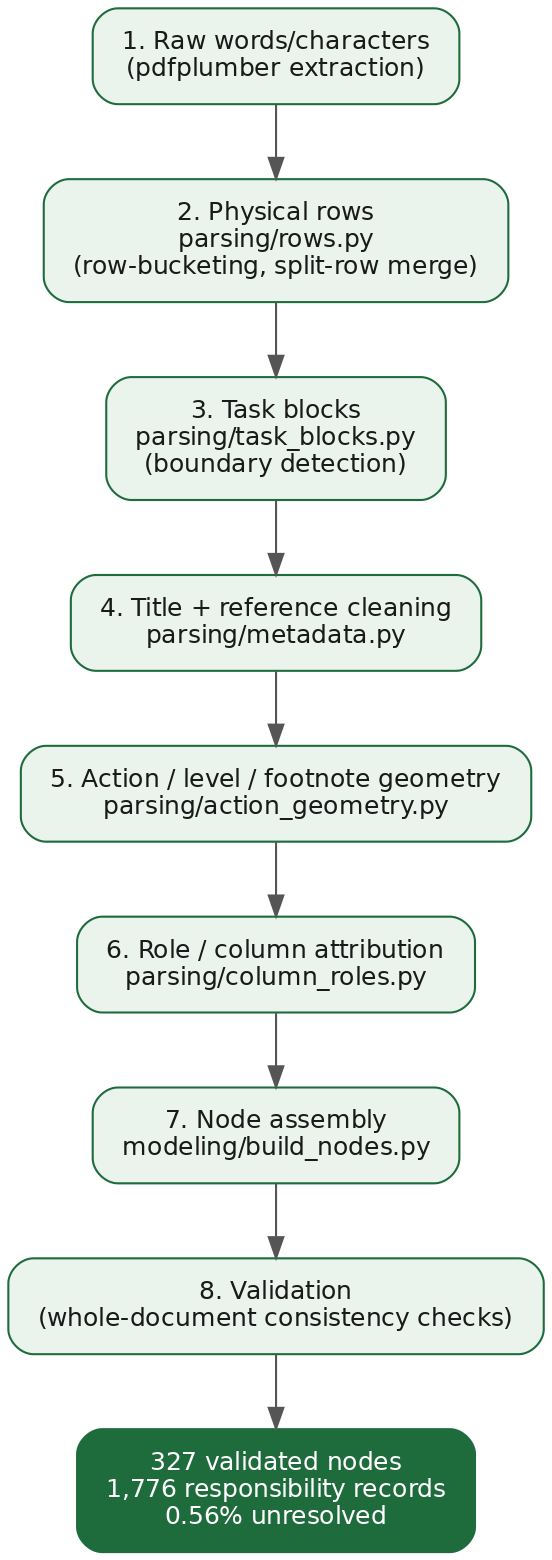
\includegraphics[width=0.82\textwidth,height=0.8\textheight,keepaspectratio]{figures/fig2_pipeline.png}
\caption{The eight-stage data preparation pipeline, from raw PDF extraction to a validated node set.}
\label{fig:fig2_pipeline}
\end{figure}
\section{Title and boundary detection}
A task's title can wrap onto a line that physically appears after its own action-code row, immediately before the *next* task's bare identifier — which a naive parser reads as belonging to the next task. The correct rule, arrived at only after two earlier attempts failed on real counter-examples, treats a task as "closed" (safe to forward-attach a following title line to the *next* task instead) only when one of three independent signals is present: a trailing period on the currently open task's text, or a second batch of action codes arriving while the current task already has some of its own. Each of the three signals was added in response to one specific, confirmed real failure (tasks 2.126, and 3.225/3.226), not designed upfront.

\section{Reference and footnote cleaning}
Cross-reference phrases ("See DAM 16.100, 16.200...") and footnote-qualification digits share the same superficial shape — bare numbers — as ordinary content, so an early version of the footnote-stripping regex was corrupting genuine reference ids and genuine dollar/UA amounts (e.g. "2,000,000" became ",,,"; "a 3-Year Rolling Business Plan" lost its "3"). The eventual, tested rule excludes a bare number from footnote-stripping whenever it is immediately preceded *or* followed by a comma or hyphen — arrived at incrementally as each new false-positive shape was discovered on real titles, and validated in \texttt{tests/\allowbreak{}test\_\allowbreak{}metadata.py} against every previously-fixed case simultaneously so a new fix could never silently reintroduce an old bug.

References themselves are extracted through four distinct regex patterns, one per real phrasing found in the document (Section 6.2), each wired into both the extraction path (so the redirect is captured in \texttt{node.references}) and the stripping path (so the same phrase does not simultaneously get mangled by the footnote-digit stripper) — the same two-sided pattern applied consistently as each new phrasing was found.

\section{Action, level, and footnote geometry}
Building on the alignment rule established in Data Understanding (Section 6.2), \texttt{parsing/\allowbreak{}action\_\allowbreak{}geometry.py} compares each small superscript character following an authority-code letter to that letter's own top and bottom edge: a digit aligned to the letter's bottom is a seniority-level indicator (at most one per code); consecutive digits aligned to the letter's top concatenate into a multi-digit footnote reference number. Anchor detection (finding the authority-code letter itself among all the small text on a page) went through three iterations to correctly exclude OCR-style letter-spaced prose ("A p p r a is a l") and isolated single letters embedded in unrelated words, each iteration validated against a specific real false-positive found on document page 12.

The "(i)" informed-marker bug (Section 6.2) — a five-character sequence including internal spaces, originally scanned for as three consecutive non-space characters — was the single fix with the largest measured impact in the entire parsing pipeline: it had silently prevented 174 of 276 informed-party markers in the previous version of this project from ever resolving to a real role.

\section{Role/column attribution}
Rotated column headers are read in descending-top character order and clustered in two passes: a tight pass (gap ≤ 3pt) groups each physical vertical text run in the correct reading order first, then a wider pass (gap ≤ 14pt, calibrated against real measured gaps: wrapped lines of the same header sit roughly 10–12pt apart, while distinct columns sit roughly 19–27pt apart) concatenates runs into full header strings. Skipping the tight pass and going straight to the wide pass was tried and rejected, because it interleaves two headers character-by-character when their y-ranges happen to overlap (a real, confirmed failure mode, not a hypothetical one).

Once headers are extracted, each authority-code cell is matched to the nearest column header by x-position (maximum 20pt distance; no match within that distance returns "unresolved" rather than a guessed wrong role). Across the full 79-page document this resolves 98.8\% of actions to a role on pages where headers exist; 43 of 79 pages have no rotated header text at all, of which 42 are legitimately non-table pages and exactly one is a genuine multi-page table continuation, handled by carrying the previous page's header set forward.

Two further real bugs were found and fixed only by checking results across the *whole* document rather than a single sample page: character interleaving between two columns sitting closer together (≈2pt) than the tight-cluster threshold on one specific page, and a false merge of two genuinely different columns caused by that same page's unusually tight spacing defeating a purely gap-based merge rule. The second was fixed with a content-based signal — stop merging once accumulated header text already ends in a balanced closing parenthesis — checked against all 79 pages before being trusted, since it changed output on only the four pages that needed it and no others.

Footnote digits trailing directly on role-header strings (e.g. "Regional NSO Lead2") were stripped only after three attempts: the first never fired at all (it checked the literal last character, which is almost always a positioned trailing space, not the digit); the second stripped only one digit of a genuine multi-digit footnote number; the third correctly excludes legitimate department codes that also end in a digit ("Manager FIFC.4") by checking that the character immediately preceding the digit run is not a literal period.

\section{Node assembly and validation}
\texttt{modeling/\allowbreak{}build\_\allowbreak{}nodes.py} performs one page-walk producing a fully enriched, typed \texttt{schema.Node} for every task, child task, and threshold variant, merged with a separate chapter/process skeleton (\texttt{modeling/\allowbreak{}hierarchy\_\allowbreak{}skeleton.py}) for the two hierarchy levels the row-level parser never directly emits. Validation was not a one-time check but a repeated, whole-document consistency pass: a \texttt{get\_\allowbreak{}children()} bug that silently returned wrong results for two of the four hierarchy levels (because it guessed parent/child relationships from id-string prefixes, which happens to work for two levels and is simply wrong for the other two) was caught only by a consistency check requiring every node's children to be of the expected type and every child's parent-pointer to point back correctly — not by manual inspection, which had missed it.

The final, current build produces \textbf{327 nodes} (3 chapters, 35 processes, 138 tasks, 102 child tasks, 49 threshold variants) and \textbf{1,776 extracted responsibility records}, with an unresolved-role rate of \textbf{0.56\%} (10 of 1,786 gross action instances) and 3 residual exact-duplicate responsibilities, all localized to one page with unusually tight column spacing and left as a small, understood residual rather than chased further. Two pre-existing empty titles (activities 2.516 and 2.522) and one residual title-corruption case (2.222.1, down from six before the character-level title-recovery fix) remain, both explicitly documented as known, bounded data-quality limitations rather than silently hidden.

\section{A chain of six real bugs from one scoping question}
Before starting work on the knowledge graph, a scoping question was raised that could have been treated as a quick sanity check: role-header strings carry a trailing footnote digit ("Regional NSO Lead2"), and action cells carry their own footnote digits — is that the same footnote numbering pool, or two separate ones? Answering it properly, against real document evidence rather than by assumption, opened a chain of six further real bugs, each found and fixed only because the previous one was checked thoroughly enough to expose the next. They are narrated here in the order found, because the chain itself — not just the individual fixes — illustrates how deceptively deep a single "quick check" question could go in this document.

\textbf{1. The footnote pools were confirmed to be the same one.} Checking a specific real table (the NSO section) directly confirmed that a role header's trailing footnote digit and an action cell's trailing footnote digit reference the same numbered list at the bottom of the table — one shared numbering pool per table, not two independent ones.

\textbf{2. A hard alignment-tolerance cutoff was silently dropping real footnote digits.} While confirming point 1, one specific authority code's footnote digit was found to sit 0.004 points past the alignment-tolerance cutoff used to distinguish a footnote digit from a seniority-level digit (Section 6.2's alignment rule) — close enough that it satisfied neither rule and was silently dropped rather than misclassified. Checked document-wide rather than patched for the one case: 30 of 345 digit decorations were being dropped this way, 23 sharing the exact same near-miss signature and 7 genuinely unrelated. The tolerance was widened from 1.5 to 2.0 points, and the two original real examples that had calibrated the 1.5 figure in the first place were re-checked to confirm they remained correctly classified under the new, looser threshold.

\textbf{3. A genuine PDF row-splitting quirk, confirmed by a requested screenshot.} Investigating a related discrepancy required requesting and inspecting a screenshot of the real table, which revealed that a wide table row's own approval-code cells could render on a *different* row-bucket than its own identifier cell — a real PDF layout quirk where the rightmost cells of a wide row land roughly a point away from the leftmost cells, enough to round into a different row grouping. This was systematic across the entire table, not an isolated case, cascading each row's action codes one position off from where they belonged. A first, broad fix (merge any two row-buckets within five points that share no overlapping word x-ranges) was tried and rejected after being checked against the whole document: it produced 1,614 candidate merges, several of them unsafe, including one case that would have spliced two unrelated activities' text together. The eventual fix used a narrower, safer signal instead — only merge a row-bucket into its neighbor if the row consists *entirely* of action-code content, since no genuine standalone table row is ever composed of nothing but authority codes.

\textbf{4. A bug in the fix for point 3, caught while testing point 3.} The new "is this row pure action-code content" check used a pattern-matching function that could not correctly recognize codes like "I2" or "I3" due to a subtle word-boundary mismatch between a letter and an immediately following digit — a normalization step that already existed elsewhere in the codebase for exactly this reason was not applied consistently in the new check, causing it to silently skip merging rows it should have merged. The fix was to reuse the existing, already-correct normalization function rather than write a second, independently-maintained version of the same logic — the same single-source-of-truth lesson the project had already learned once (Section 6.3), this time self-inflicted rather than found in the source PDF.

\textbf{5. A second occurrence of the comma-adjacency footnote bug, this time via a hyphen.} Fixing point 3 surfaced a real activity title for the first time that had previously been hidden behind the row-splitting bug, and it was corrupted: "Concerned Staff members below PL-2 level" had lost its digit, rendering as "...below PL- level". The cause was a near-miss of a bug already fixed once before (Section 6.3's comma-adjacency exclusion for footnote-digit stripping): the existing rule excluded a bare digit immediately preceded by a comma or hyphen, but did not exclude one immediately *followed* by a hyphen, and "PL-2" has exactly that shape. Checked document-wide before extending the rule (six affected blocks found, five genuinely fixed by the extension, one pre-existing unrelated garbling left untouched) rather than assumed to be an isolated case.

\textbf{6. A geometry search-window bug, caught only while writing the regression test for point 3.} After the row-merge fix from point 3, the merged rows' *text* was correct, but their *authority-code actions* had vanished entirely. The cause traced to a helper function that reported a row-bucket's vertical span as a single repeated point value rather than the true minimum and maximum vertical extent of the words actually inside it — harmless before the row-merge fix existed, since an unmerged row's words were always within about a point of that single value anyway, but no longer harmless once a merged row could legitimately span several points, which then fell outside the small fixed search window the geometry-based action extractor used to look for authority codes near a given row. The fix made the helper report the row's genuine vertical span, correct for merged rows and a no-op for the unmerged case.

Following this chain, a full re-test confirmed all pre-existing tests still passed, five new regression tests were added pinning the exact values recovered from the requested screenshot, and a full document rebuild showed total extracted responsibilities rising from 937 to 1,776 — the row-splitting fix alone recovering a substantial number of real actions that had previously been silently dropped or misattributed across roughly two dozen affected rows document-wide.

